\begin{figure*}[t]
    \centering
    % \includegraphics[width=\linewidth]{figures/pdf_files/method_v2.pdf}
    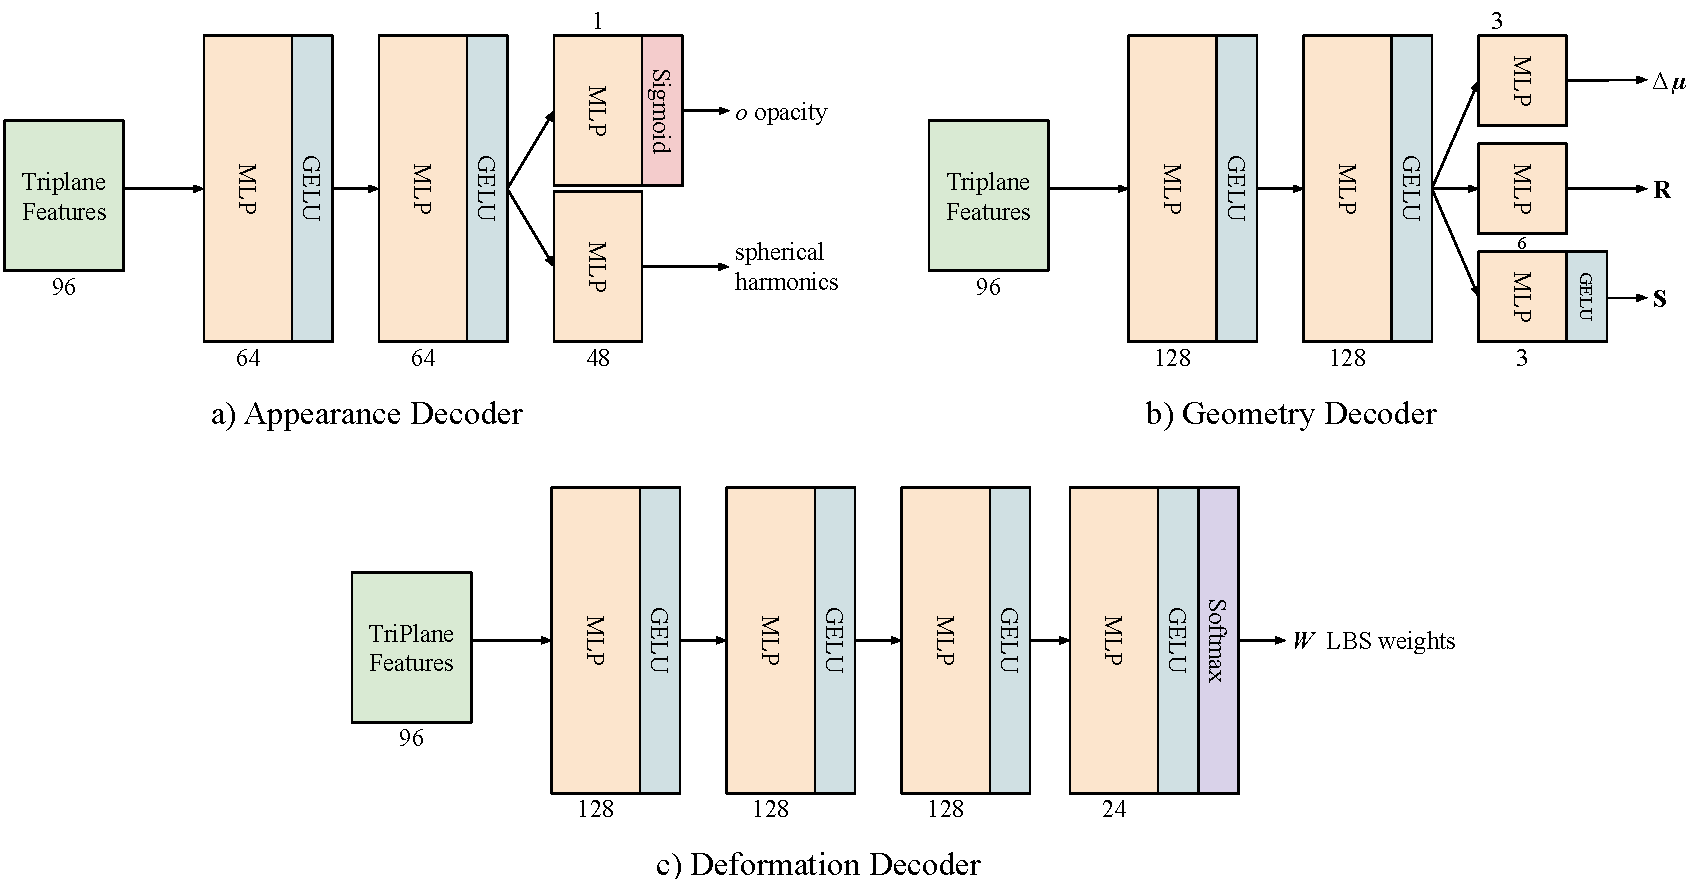
\includegraphics[width=\linewidth]{figures/pdf_files/network_architecture.pdf}
    \vspace{-7mm}
    \caption{\textbf{\acronym model architecture.} Here we show the network architecture of decoder models. 
    Appearance decoder $D_A$ is a 2-layer MLP with GELU~\cite{hendrycks2016gelu} activations. It takes triplane features as input and outputs opacity \& spherical harmonics parameters. Sigmoid activation function is used for opacity to constrain the values between $[0, 1]$. Geometry decoder $D_G$ also uses 2-layer MLP with GELU activation. It outputs the $\Delta \bm{\mu}, \bm{R}, \bm{S}$ for each Gaussians. We use GELU activation to ensure $\bm{S} \ge 0$. We do not need a normalization activation for $R$ unlike Kerbl \etal~\cite{kerbl3Dgaussians} since we use 6D rotation representation. We use a 3-layer MLP for deformation decoder $D_D$. It outputs the LBS weights. We apply a low-temperature softmax activation function with $T=0.1$ to ensure $\sum_{k=1}^{n_k} W_{k,i} = 1$. The use of a low temperature assists in predicting unimodal distributions, as most Gaussians need to be assigned to a single bone transformation.
    }
    \label{fig:netarch}
    \vspace{-2ex}
\end{figure*}{}